% ------------------------------------------------------------------------------
% Chapter 3
% ------------------------------------------------------------------------------
\chapter{ Heading ofr Chapter 3} % enter the name of the chapter here
\label{cha:chapter 3 label} % enter the chapter label here (for cross referencing)
\begin{equation}
    \label{eu_eqn}
    e^{\pi i } +1 =0
\end{equation}

\begin{equation}
    \label{eu_eqn}
    e^{\pi i } +2 =0
\end{equation}

\begin{equation} \label{eq1}
\begin{split}
A & = \frac{\pi r^2}{2} \\
 & = \frac{1}{2} \pi r^2
\end{split}
\end{equation}

\begin{table}
\centering
\caption{Table's caption goes here}
\begin{tabular}{|l|l|l|l|} 
\hline
Col1 & Col2 & Col3 & Col4  \\ 
\hline
21   & 22   & 23   & 24    \\ 
\hline
31   & 32   & 33   & 34    \\
\hline
\end{tabular}
\end{table}

This is a citation example \cite{rusk2016deep}

\begin{figure}
    \centering
    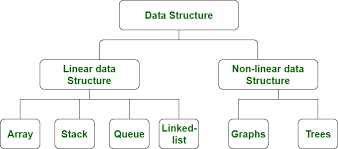
\includegraphics[width = 0.6\textwidth]{Images/ds.png}
    \caption{Data Structures}
    \label{fig:ds}
\end{figure}

\begin{itemize}
    \item Chapter \ref{cha:chapter 2 label}
    \item Table \ref{tab:table label}
\end{itemize}

\begin{enumerate}
    \item First Item
    \item Second
    \begin{enumerate}
        \item Subsection
        \item Subsection2 
    \end{enumerate}
\end{enumerate}

\blindtext[2]